%package list
\documentclass{article}
\usepackage[top=3cm, bottom=3cm, outer=3cm, inner=3cm]{geometry}
\usepackage{multicol}
\usepackage{graphicx}
\usepackage{url}
%\usepackage{cite}
\usepackage{hyperref}
\usepackage{array}
%\usepackage{multicol}
\newcolumntype{x}[1]{>{\centering\arraybackslash\hspace{0pt}}p{#1}}
\usepackage{natbib}
\usepackage{pdfpages}
\usepackage{multirow}
\usepackage[normalem]{ulem}
\useunder{\uline}{\ul}{}
\usepackage{svg}
\usepackage{xcolor}
\usepackage{listings}
\lstdefinestyle{ascii-tree}{
    literate={├}{|}1 {─}{--}1 {└}{+}1 
  }
\lstset{basicstyle=\ttfamily,
  showstringspaces=false,
  commentstyle=\color{red},
  keywordstyle=\color{blue}
}
%\usepackage{booktabs}
\usepackage{caption}
\usepackage{subcaption}
\usepackage{float}
\usepackage{array}

\newcolumntype{M}[1]{>{\centering\arraybackslash}m{#1}}
\newcolumntype{N}{@{}m{0pt}@{}}


%%%%%%%%%%%%%%%%%%%%%%%%%%%%%%%%%%%%%%%%%%%%%%%%%%%%%%%%%%%%%%%%%%%%%%%%%%%%
%%%%%%%%%%%%%%%%%%%%%%%%%%%%%%%%%%%%%%%%%%%%%%%%%%%%%%%%%%%%%%%%%%%%%%%%%%%%
\newcommand{\itemStudent}{Andre Renzo Añasco Huamanquispe}
\newcommand{\itemStudentc}{Frank's Javier Vilca Quispe }
\newcommand{\itemStudenta}{Jhamil Yeider Turpo Añasco}
\newcommand{\itemStudentb}{Melsy Melani Huamani Vargas}
\newcommand{\itemCourse}{Programación}
\newcommand{\itemCourseCode}{20231001}
\newcommand{\itemSemester}{I}
\newcommand{\itemUniversity}{Universidad Nacional de San Agustín de Arequipa}
\newcommand{\itemFaculty}{Facultad de Ingeniería de Producción y Servicios}
\newcommand{\itemDepartment}{Departamento Académico de Ingeniería de Sistemas e Informática}
\newcommand{\itemSchool}{Escuela Profesional de Ingeniería de Sistemas}
\newcommand{\itemAcademic}{2023 - A}
\newcommand{\itemInput}{Del 30 junio 2023}
\newcommand{\itemOutput}{Al 05 agosto 2023}
\newcommand{\itemPracticeNumber}{Trabajo Final}
\newcommand{\itemTheme}{Trabajo Final}
%%%%%%%%%%%%%%%%%%%%%%%%%%%%%%%%%%%%%%%%%%%%%%%%%%%%%%%%%%%%%%%%%%%%%%%%%%%%
%%%%%%%%%%%%%%%%%%%%%%%%%%%%%%%%%%%%%%%%%%%%%%%%%%%%%%%%%%%%%%%%%%%%%%%%%%%%

\usepackage[english,spanish]{babel}
\usepackage[utf8]{inputenc}
\AtBeginDocument{\selectlanguage{spanish}}
\renewcommand{\figurename}{Figura}
\renewcommand{\refname}{Referencias}
\renewcommand{\tablename}{Tabla} %esto no funciona cuando se usa babel
\AtBeginDocument{%
	\renewcommand\tablename{Tabla}
}

\usepackage{fancyhdr}
\pagestyle{fancy}
\fancyhf{}
\setlength{\headheight}{30pt}
\renewcommand{\headrulewidth}{1pt}
\renewcommand{\footrulewidth}{1pt}
\fancyhead[L]{\raisebox{-0.2\height}{
\includegraphics[width=3cm]{img/logo_episunsa.png}}}
\fancyhead[C]{\fontsize{7}{7}\selectfont	\itemUniversity \\ \itemFaculty \\ \itemDepartment \\ \itemSchool \\ \textbf{\itemCourse}}
\fancyhead[R]{\raisebox{-0.2\height}{
\includegraphics[width=1.2cm]{img/logo_abet}}}
\fancyfoot[C]{\itemCourse}
\fancyfoot[R]{Página \thepage}

% para el codigo fuente
\usepackage{listings}
\usepackage{color, colortbl}
\definecolor{dkgreen}{rgb}{0,0.6,0}
\definecolor{gray}{rgb}{0.5,0.5,0.5}
\definecolor{mauve}{rgb}{0.58,0,0.82}
\definecolor{codebackground}{rgb}{0.95, 0.95, 0.92}
\definecolor{tablebackground}{rgb}{0.8, 0, 0}

\lstset{frame=tb,
	language=bash,
	aboveskip=3mm,
	belowskip=3mm,
	showstringspaces=false,
	columns=flexible,
	basicstyle={\small\ttfamily},
	numbers=none,
	numberstyle=\tiny\color{gray},
	keywordstyle=\color{blue},
	commentstyle=\color{dkgreen},
	stringstyle=\color{mauve},
	breaklines=true,
	breakatwhitespace=true,
	tabsize=3,
	backgroundcolor= \color{codebackground},
}

\begin{document}
	
	\vspace*{10px}
	
	\begin{center}	
		\fontsize{17}{17} \textbf{ Informe de Laboratorio \itemPracticeNumber}
	\end{center}
	\centerline{\textbf{\Large Tema: \itemTheme}}
	%\vspace*{0.5cm}	

	\begin{flushright}
		\begin{tabular}{|M{2.5cm}|N|}
			\hline 
			\rowcolor{tablebackground}
			\color{white} \textbf{Nota}  \\
			\hline 
			     \\[30pt]
			\hline 			
		\end{tabular}
	\end{flushright}	

	\begin{table}[H]
		\begin{tabular}{|x{4.7cm}|x{4.8cm}|x{4.8cm}|}
			\hline 
			\rowcolor{tablebackground}
			\color{white} \textbf{Estudiante} & \color{white}\textbf{Escuela}  & \color{white}\textbf{Asignatura}   \\
			\hline 
			{\itemStudent \par \itemStudenta \par \itemStudentb \par \itemStudentc} & \itemSchool & {\itemCourse \par Semestre: \itemSemester \par Código: \itemCourseCode}     \\
			\hline 			
		\end{tabular}
	\end{table}		
	
	\begin{table}[H]
		\begin{tabular}{|x{4.7cm}|x{4.8cm}|x{4.8cm}|}
			\hline 
			\rowcolor{tablebackground}
			\color{white}\textbf{Laboratorio} & \color{white}\textbf{Tema}  & \color{white}\textbf{Duración}   \\
			\hline 
			\itemPracticeNumber & \itemTheme & 04 horas   \\
			\hline 
		\end{tabular}
	\end{table}
	
	\begin{table}[H]
		\begin{tabular}{|x{4.7cm}|x{4.8cm}|x{4.8cm}|}
			\hline 
			\rowcolor{tablebackground}
			\color{white}\textbf{Semestre académico} & \color{white}\textbf{Fecha de inicio}  & \color{white}\textbf{Fecha de entrega}   \\
			\hline 
			\itemAcademic & \itemInput &  \itemOutput  \\
			\hline 
		\end{tabular}
	\end{table}
	
	\section{Tipos de Datos:}
	\begin{itemize}		
		\item La página web que diseñamos es útil para la cafetería Caffe.Aqp con una óptima interacción humano-computadora y características centradas en la eficiencia operativa y la satisfacción del cliente tiene el potencial de revolucionar la forma en que las cafeterías gestionan sus operaciones y brindan servicios a sus clientes. La plataforma ofrece una solución integral que beneficia tanto a los administradores como a los clientes, creando una experiencia más conveniente y placentera en todos los aspectos. La página web se ha desarrollado con el propósito de optimizar la gestión de productos, pedidos, reservas de mesas y la generación de boletas.
	\end{itemize}
		
	\section{Requisitos del sistema}
	\begin{itemize}
		\item El sistema debe satisfacer los siguientes requisitos funcionales y no funcionales:
		\item RQ01 : El sistema debe estar disponible en Internet a través de una URL.
		\item RQ02 : El sistema debe permitir el inicio/cierre de sesión.
		\item RQ03 : El sistema debe permitir gestionar los productos ingresados y los eliminados solo a los administradores.
		\item RQ04 : El sistema debe permitir poder configurar cada uno de los atributos de los productos solo a los administradores.
		\item RQ05 : El sistema debe permitir realizar reservaciones para cada uno de los clientes..
		\item RQ06 : El sistema debe permitir realizar compras en línea.
  	\item RQ07: El sistema debe enviar 
        notificaciones por correo electrónico, cuando se realice una compra.
		\item RQ08: El sistema debe ser compatible con dispositivos móviles.
	\end{itemize}
	
	\section{Modelado de datos}
	\begin{itemize}
		\item El modelo de comidas: En esta entidad se guardarán cada uno de los productos ingresados. Los atributos por los que estará compuesto esta entidad son: id, que será su código único, name el cual será el nombre del producto, tipos el cual indicará si es bebida comida o postre, imagen para poder guardar una imagen en el, desc la cual es una breve descripción del producto y por último price que será el precio del producto.
        \begin{lstlisting}[language=bash,caption={Modelado de comidas}][H]
		class comidas(models.Model):
           id = int
           name = models.CharField(max_length=100)
           tipo = models.CharField(max_length=2, choices=Tipo, default='4')
           img = models.ImageField(upload_to='pics')
           desc = models.TextField(default='')
           price = models.IntegerField()

  	\end{lstlisting}
		\item El modelo de  clientes: En esta entidad se guardaran los clientes que ingresamos en nuestra bd. Los atributos que contendrá nuestra entidad son nombre, el cual obtendrá el nombre de este, email, el cual contendrá su email donde se enviará su boleta de compra y por último su teléfono para poder comunicarnos con el.
        \begin{lstlisting}[language=bash,caption={Modelo de clientes}][H]
		
       class Cliente(models.Model):
          nombre = models.CharField(max_length=100)
          email = models.EmailField()
          telefono = models.CharField(max_length=20)

        def __str__(self):
            return self.nombre
    
        class Meta:
            ordering = ['nombre']

        def get_absolute_url(self):
            return reverse('cliente-detail', args=[str(self.id)])
	  \end{lstlisting}
		\item El modelo de Pedido: En esta entidad podremos guardar los valores de los Pedidos realizados, comenzando por el cliente el cual realizó dicho pedido, la fecha en la que se adquirió el pedido y los productos adquiridos, También tendrá un modelo de nombre ESTADOSPEDIDO, para saber si esta pendiente, ya se esta realizando o se completo.
        \begin{lstlisting}[language=bash,caption={Modelo de pedido}][H]
		class Pedido(models.Model):
              cliente = models.ForeignKey('Cliente', on_delete=models.CASCADE)
              fecha = models.DateTimeField(auto_now_add=True)
              productos = models.ManyToManyField('Producto', through='ItemPedido')
            ESTADOS_PEDIDO = [
                ('P', 'Pendiente'),
                ('E', 'En preparación'),
                ('C', 'Completado'),
            ]
             estado = models.CharField(max_length=1, choices=ESTADOS_PEDIDO, default='P')

             def __str__(self):
                 return f"Pedido {self.cliente} - {self.id}"

	  \end{lstlisting}
		\item El modelo ITEMPEDIDO: Esta entidad viene a ser de relación, entre producto y pedido, donde tendrá el llamado de ambas tablas y se le añadirá el valor de cantidad.
        \begin{lstlisting}[language=bash,caption={Modelo ITEMPEDIDO}][H]
	      class ItemPedido(models.Model):
                pedido = models.ForeignKey('Pedido', on_delete=models.CASCADE)
                producto = models.ForeignKey('Producto', on_delete=models.CASCADE)
                cantidad = models.PositiveIntegerField()

                def subtotal(self):
                    return self.cantidad * self.producto.precio

                def __str__(self):
                return f"Pedido {self.producto.nombre}, Cantidad {self.cantidad}, Precio unitario {self.producto.precio}"
	  \end{lstlisting}
        \item El modelo carrito: Esta entidad será de referencia para saber qué productos se adquirió.
        \begin{lstlisting}[language=bash,caption={Modelo de carrio}][H]
		    class Carrito(models.Model):
                cliente = models.OneToOneField('Cliente', on_delete=models.CASCADE)
                productos = models.ManyToManyField('Producto', through='ItemCarrito')

                def __str__(self):
                    return f"Carrito de {self.cliente.nombre}"
	  \end{lstlisting}
        \item El modelo ReservaMesa: Esta entidad sirve para poder guardar la información de las mesas que serán reservadas, se guardará el cliente, la fecha en la que se hará la reserva, la hora en la que se acercara el cliente, y la cantidad de personas que asistiran.
        \begin{lstlisting}[language=bash,caption={Modelo de ReservaMesa}][H]
		     class ReservaMesa(models.Model):
                cliente = models.ForeignKey('Cliente', on_delete=models.CASCADE)
                fecha = models.DateField()
                hora = models.TimeField()
                cantidad_personas = models.PositiveIntegerField()

                def __str__(self):
                    return f"Reserva para {self.cantidad_personas} personas el {self.fecha} a las {self.hora}"
	  \end{lstlisting}
  
	\end{itemize}
		
	\section{Diccionario de datos}
	\begin{itemize}
		\item \textbf{Categoria:}
	
	Campos: nombre, descripcion
	Descripción: Este modelo almacena información sobre las categorías de productos disponibles en la cafetería. Cada categoría tiene un nombre y una descripción.
	\begin{figure}[h!]
		\centering
		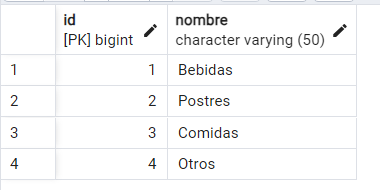
\includegraphics[width=1\linewidth]{img/tcategoria}
		\caption{Tabla de categoria}
		\label{fig:tcategoria}
	\end{figure}
	
		\item \textbf{Producto:}
	
	Campos: categoria, nombre, descripcion, precio, imagen
	Descripción: El modelo de Producto guarda detalles sobre los productos ofrecidos en la cafetería. Cada producto está asociado a una categoría y tiene un nombre, descripción, precio y una imagen.
	\begin{figure}[h!]
		\centering
		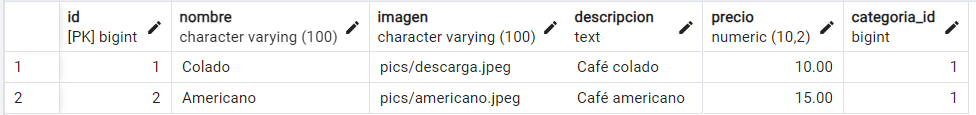
\includegraphics[width=1\linewidth]{img/tproducto}
		\caption{Tabla producto}
		\label{fig:tproducto}
	\end{figure}
	
		\item \textbf{Cliente:}
	
	
	Campos: nombre, apellido, correo, telefono
	Descripción: El modelo de Cliente almacena información de los clientes que visitan la cafetería. Incluye el nombre, apellido, correo electrónico y número de teléfono de los clientes.
	\begin{figure}[h!]
		\centering
		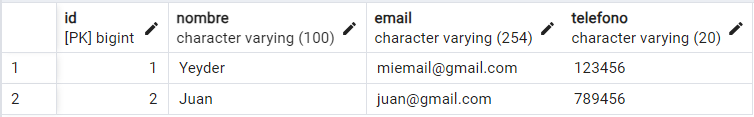
\includegraphics[width=1\linewidth]{img/tcliente}
		\caption{tabla de cliente}
		\label{fig:tcliente}
	\end{figure}
	
		\item \textbf{Pedido:}
		
		Campos: cliente, producto, fecha-pedido, estado
		Descripción: El modelo de Pedido registra los pedidos realizados por los clientes. Cada pedido tiene un cliente asociado, un producto solicitado, la fecha del pedido y su estado (pendiente, entregado, etc.).
		\begin{figure}[h!]
			\centering
			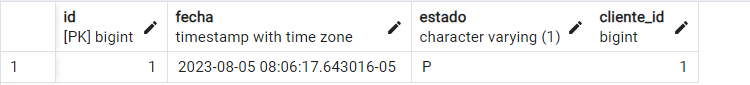
\includegraphics[width=1\linewidth]{img/tpedido}
			\caption{Tabla pedido}
			\label{fig:tpedido}
		\end{figure}
		
	
		\item \textbf{itemPedido:}
	
	Campos: pedido, cantidad
	Descripción: El modelo de DetallePedido guarda información sobre los productos y las cantidades asociadas a un pedido específico. Cada detalle de pedido está vinculado a un pedido y registra la cantidad de un producto solicitado.
	\begin{figure}[h!]
		\centering
		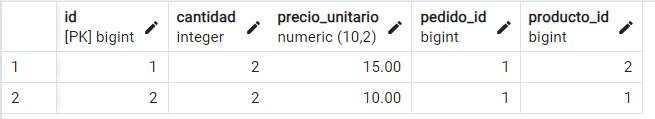
\includegraphics[width=1\linewidth]{img/titempedido}
		\caption{Tabla itemPedido}
		\label{fig:titempedido}
	\end{figure}
	
		\item \textbf{Carrito:}
		
	Campos: cliente
	Descripción: El modelo "Carrito" representa el carrito de compras de un cliente. Está asociado a un cliente específico y actúa como un contenedor temporal para los productos que el cliente planea comprar.
	\begin{figure}[h!]
		\centering
        
		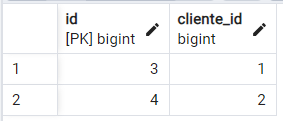
\includegraphics[width=0.5\linewidth]{lab01/latex/img/tcarrito.png}
		\caption{Tabla carrito}
		\label{fig:tcarrito}
	\end{figure}

        \newpage
		\item \textbf{ItemCarrito:}
		
	Campos: carrito, producto, cantidad
	Descripción: El modelo "ItemCarrito" registra los productos y las cantidades agregadas al carrito de compras de un cliente. Cada elemento del carrito está vinculado a un carrito, un producto específico y la cantidad deseada.
	\begin{figure}[h!]
		\centering
		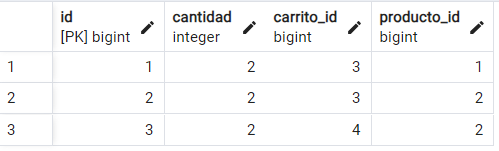
\includegraphics[width=.75\linewidth]{img/titemcarrito}
		\caption{Tabla itemCarrito}
		\label{fig:titemcarrito}
	\end{figure}
	
	\end{itemize}
		
	\section{Diagrama Entidad-Relación (ERD)}
	En esta sección se mostrará los modelos creados con sus respectivos campos en el proyecto y la relación entre cada uno de ellos.
	
	Inicialmente se mostrará cada uno de las tablas y sus relaciones, para una mejor comprensión, las tablas genteradas son: categoria, producto, cliente, carrito, pedido, itemcarrito e itempedido.
	
	\subsection{modelo categoria}
	Consta de un campo "nombre" y tiene una relación de uno a muchos con el modelo producto, esto porque una categoría (bebidas, postres y entre otros) pueden tener muchos productos.
	\begin{figure}[h!]
		\centering
		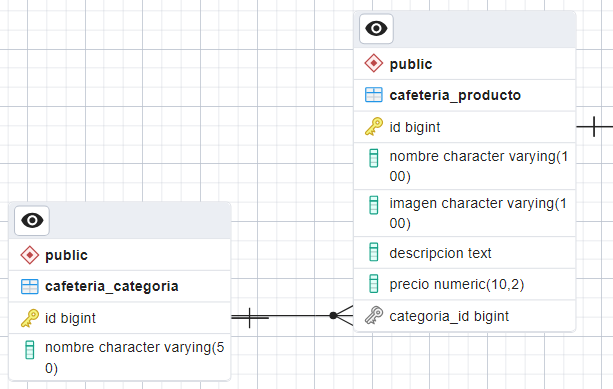
\includegraphics[width=.7\linewidth]{img/modCategoria}
		\caption{Figura de del modelo categoria y sus relaciones}
		\label{fig:modcategoria}
	\end{figure}
	
	\subsection{modelo producto}
	Consta de de campos como nombre, imagen, descripción, precio y tiene una relación de mushos a uno con categoría, como se explicó anteriormente, y también tiene una relación de uno a muchos con itemcarrito e itempedido (ambos).
	\begin{figure}[h!]
		\centering
		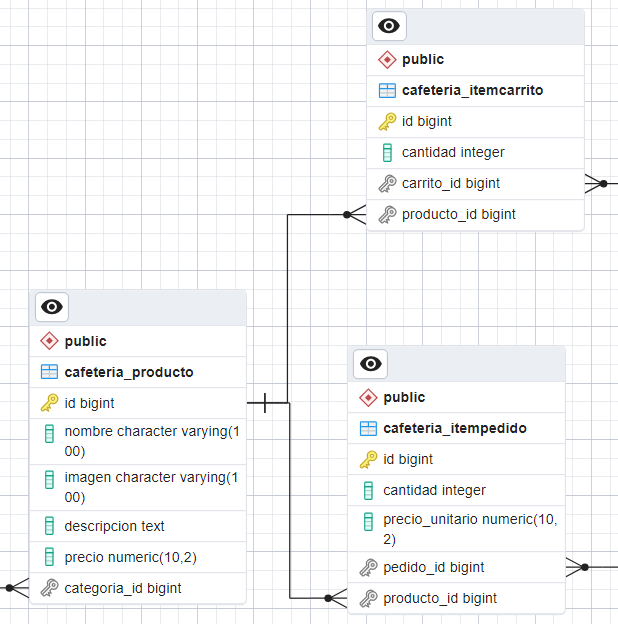
\includegraphics[width=.5\linewidth]{img/modProducto}
		\caption{Figura de del modelo producto y sus relaciones}
		\label{fig:modproducto}
	\end{figure}
	\newpage
	\subsection{modelo cliente, carrito, pedido}
	El modelo cliente consta de campos como nombre, email y telefono, y tiene  una relación de uno a muchos con carrito e edido (ambos). A su vez el modelo carrito tiene una relación de uno a muchos con el modelo itemcarrito, puede tene muchos itme carrito que su su vez guardan productos. Por otro lado, el modelo pedido también tiene una relación de uno a muchos con el modelo itempedido, y esta guarda a productos.
	\begin{figure}[h!]
		\centering
		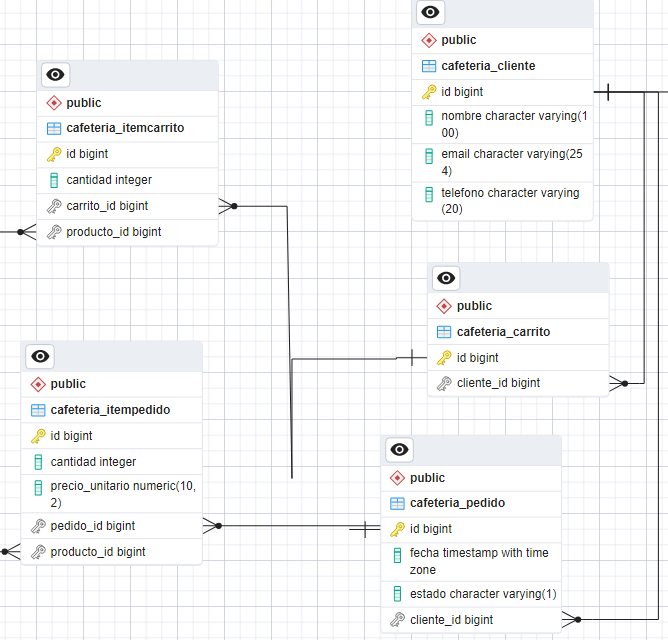
\includegraphics[width=1\linewidth]{img/modClienteotros}
		\caption{Figura de del modelo cliente, carrito y pedido con sus respactivas relaciones}
		\label{fig:modclienteotros}
	\end{figure}
	\newpage
	\subsection{modelo cliente, carrito, pedido}
	Antes de ver estos modelos, debemos tener en cuenta que estos modelos sirven como enlace a producto con carrito y pedido, esta relación inicialmente se consideraba de muchos a muchos, sin embargo, Django genera otra tabla por defecto con relación de uno a muchos. Estas tablas cumplen la misma funcionalidad y tienen algunos campos más.
	\begin{figure}[h!]
		\centering
		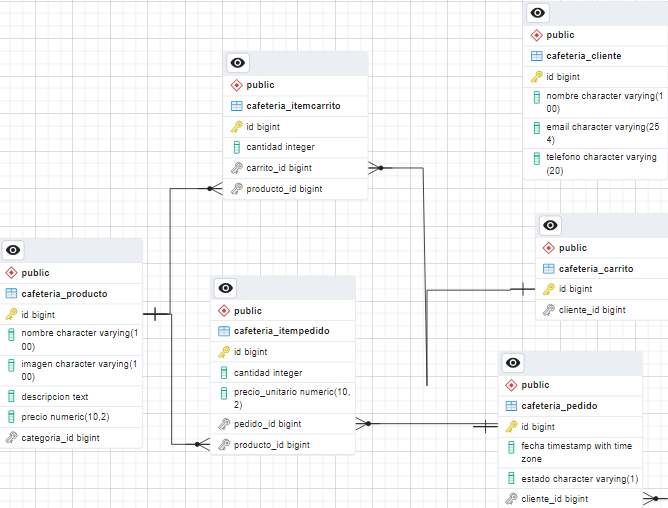
\includegraphics[width=.7\linewidth]{img/modItems}
		\caption{Figura de del modelo itemcarrito e itempedido con sus respactivas relaciones}
		\label{fig:moditems}
	\end{figure}
	\newpage
	\subsection{modelo ERD}
	Ahora se mostrará la tabla con los modelos completos y sus respectivas relaciones.
	\begin{figure}[h!]
		\centering
		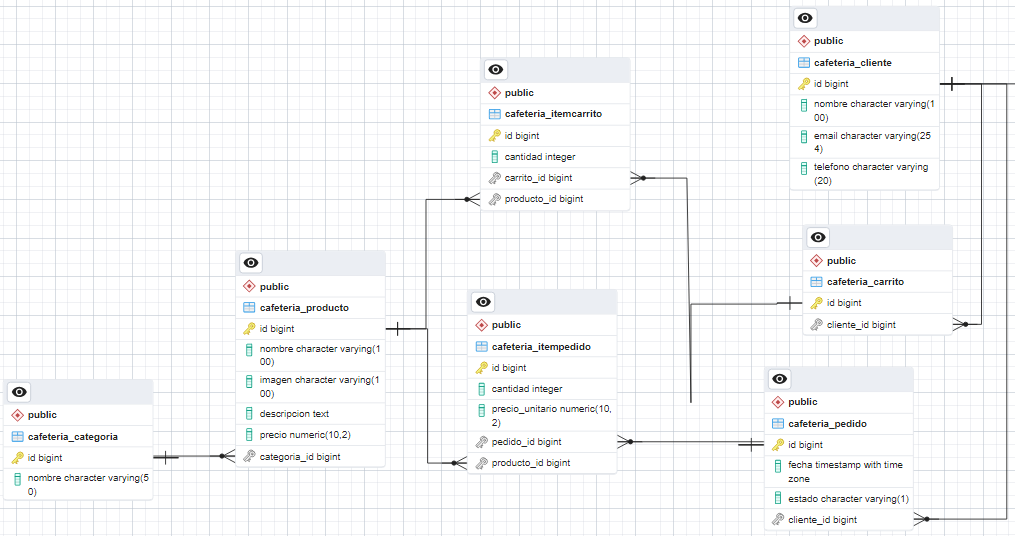
\includegraphics[width=.7\linewidth]{img/DER}
		\caption{Se puede visualizar el Diagrama Entidad Relación completo, con los 7 modelos creados en código}
		\label{fig:der}
	\end{figure}	


 \newpage
	\section{Administración con Django}
	\subsection{Setup}
\begin{enumerate}
	\item Se utilizo django como framework de trabajo
	\item Se creo un entorno virtual "n" para no tener conflictos con otros proyectos
	\item Se descargaron librerias de python con pip como:
		 \begin{itemize}
			 \item pillow
			 \item psycopg2
			 \item sqlparse
		 \end{itemize}
	\item se descargo postgres y pg admin como base de datos.
	\item se creo el proyecto con "python startproject tienda" 
\end{enumerate}
	\begin{itemize}
\section{Plantillas Bootstrap}
\begin{itemize}
	\item  Se seleccionó la siguiente plantilla para el usuario final (No administrador).
	\begin{itemize}
	\item  Demo online: Yummy
	\item URL: \href{https://bootstrapmade.com/yummy-bootstrap-restaurant-website-template/}{Link Aqui}
	\end{itemize}
Se muestran las actividades realizadas para adecuación de plantillas, vistas, formularios en Django.

	\item  Se adecuo a una carpeta static, todos aquellos elementos como su nombre lo indica, estaticos.
	
	\item  Esto incluye imagenes, hojas de estilos y javascripts.

\end{itemize}
	\begin{figure}[h]
	  \centering
	  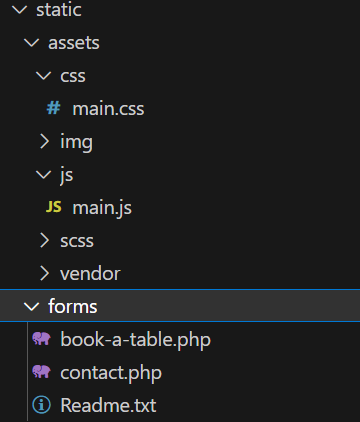
\includegraphics[width=0.6\textwidth]{lab01/latex/img/static.png}
	  \caption{Partes staticas.}
	  \label{fig:imagen-ejemplo}
	\end{figure}
	\item  Para usar los elementos de tipo dinamico se modifico usando diccionarios de contexto que permitan representar los elementos de la base de datos 
	\begin{lstlisting}

		
		
		<!-- Bebidas -->    
		<div class="row gy-5">
		  <div class="col-lg-4 menu-item">
			<img src="{{comids.img.url}}" class="menu-img img-fluid" alt="">
			<h4>{{comids.name}}</h4>
			<p class="ingredients">
			  {{comids.desc}}
			</p>
			<p class="price">
			  ${{comids.price}}
			</p>
		  </div><!-- Menu Item -->
		</div>
		
		
	\end{lstlisting}
\end{itemize}

	
\section{CRUD - Core Business - Clientes finales}
\begin{itemize}
	\item El núcleo de negocio del sistema de ventas para el restaurante radica en la facial vizualizacion de los contenidos y productos para el usuario, como el control y manejo para los miembros del staff:
	\begin{enumerate}
	\item El staff inicia sesión.
	\item Si pertenece al grupo selecto es capaz de  editar los productos.
	\item Se dirije a la pagina de agregar contenidos usando la interfaz de django.
	\item El miembro del staff vizualiza mediante las tablas, los productos previamente ingresados. 
	\item El staff es es capaz de añadir, editar o eliminar los productos. 
	\item El staff cierra sesión.

	
	\end{enumerate}
  \item Todas y cada una de estas pantallas debe funcionar en la plantilla bootstrap.
A continuación se muestran las actividades realizadas para su construcción:  
\end{itemize}

 \subsection{index.html}
	\begin{itemize}
  \item  El index.html es la primera impresión que los visitantes tienen de tu cafetería en línea. Proporciona la oportunidad de causar una impresión positiva al mostrar un diseño atractivo, imágenes de productos deliciosos y un diseño organizado que refleja la personalidad y el ambiente de tu cafetería.
		\begin{itemize}
	  \item  Navegación: El archivo index.html sirve como el centro de navegación de tu sitio. Mediante enlaces o secciones, los usuarios pueden acceder fácilmente a información esencial como los productos disponibles, la información de la cafetería, la ubicación y los precios. Esto facilita que los usuarios encuentren rápidamente lo que están buscando.
	   \item  Presentación de Productos: A través del index.html, puedes presentar tus productos de manera atractiva. Mediante imágenes de alta calidad y descripciones detalladas, puedes mostrar la variedad y calidad de los productos que ofreces, lo que puede atraer el interés y el apetito de los visitantes.
   
		\end{itemize}
	\end{itemize}

	
 \subsection{register.html}
	\begin{itemize}
  \item  La página register.html es un componente crucial en el sitio web de la cafetería, ya que permite a los visitantes registrarse y crear cuentas personalizadas
		\begin{itemize}
	  \item  Acceso Personalizado: La página de registro proporciona a los usuarios un acceso personalizado al sitio web de la cafetería. Al crear cuentas individuales, los clientes pueden disfrutar de una experiencia más rica y específica que incluye funciones como realizar pedidos en línea y comunicarse con el personal del staff.
	   \item  Recopilación de Información Esencial: Durante el proceso de registro, se recopila información clave, como nombres, direcciones de correo electrónico y nombres de usuario. Esta información permite al personal de la cafetería una forma responder a las peticiones y feedback con los clientes, brindar un servicio más orientado a sus necesidades.
	   \item  Seguridad y Autenticación: La página register.html juega un papel fundamental en la seguridad y autenticación de los usuarios. Después de registrar una cuenta, los usuarios deben iniciar sesión con sus credenciales únicas, lo que asegura que solo las personas autorizadas tengan acceso a las funciones y datos relacionados con la cuenta.
	   \item  Base de Datos de Clientes: La información recopilada durante el registro se almacena en la base de datos de PostgreSQL. Esto no solo permite la autenticación de usuarios, sino que también proporciona a la cafetería una valiosa base de datos de clientes para futuros análisis y estrategias de marketing.
			
   
		\end{itemize}
	\end{itemize}

\section{Investigación: Email, Upload.}
	\begin{itemize}
		\item Email: Se utilizará la funcionalidad del uso de envío de correos electrónicos para la parte de comunicación del usuario con el staff. Para ello se utilizo, un formulario para contactarse con los clientes y den su opinion acerca del negocio
	\end{itemize}
	\begin{lstlisting}

	<form action="forms/contact.php" method="post" role="form" class="php-email-form p-3 p-md-4">
	  <div class="row">
		<div class="col-xl-6 form-group">
		  <input type="text" name="name" class="form-control" id="name" placeholder="Your Name" required>
		</div>
		<div class="col-xl-6 form-group">
		  <input type="email" class="form-control" name="email" id="email" placeholder="Your Email" required>
		</div>
	  </div>
	  <div class="form-group">
		<input type="text" class="form-control" name="subject" id="subject" placeholder="Subject" required>
	  </div>
	  <div class="form-group">
		<textarea class="form-control" name="message" rows="5" placeholder="Message" required></textarea>
	  </div>
	  <div class="my-3">
		<div class="loading">Loading</div>
		<div class="error-message"></div>
		<div class="sent-message">Your message has been sent. Thank you!</div>
	  </div>
	  <div class="text-center"><button type="submit">Send Message</button></div>
	\end{lstlisting}
	
	\section{Video}
	\begin{itemize}			
		\item Se presenta un video con los integrantes del proyecto \href{https://drive.google.com/drive/folders/1n5q-sokJrMleBdvlblGO5rhaxiXWwcVs?usp=sharing}{Explicacion del proyecto}
	\end{itemize}

	\section{REFERENCIAS}
	
	\begin{itemize}			
		\item \url{https://bootstrapmade.com/yummy-bootstrap-restaurant-website-template/}
		\item \url{https://github.com/AndreRH09/Pweb2_ProyectoFinal.git}
		\item \url{https://www.codingforentrepreneurs.com/blog/html-template-to-pdf-in-django/}
	\end{itemize}	
	
%\clearpage
%\bibliographystyle{apalike}
%\bibliographystyle{IEEEtranN}
%\bibliography{bibliography}
			
\end{document}